
\section{Durchführung}
\label{sec:Durchführung}
\subsection{Geschwindigkeit des Wagens}
Ein Wagen ist auf einer Schiene angebracht und wird mittels Seilzug von einem
Synchronmotor angetrieben. Seine Geschwindigkeit lässt sich mit 10 verschiedenen
Gängen variieren. Wie in Abbildung \ref{fig:geschw} zu sehen.
Zur Bestimmung der Geschwindigkeit werden Weg und Laufzeit des Wagens vermessen, letztere fünf mal.
Zwei Lichtschranken, bestehend aus Phototransistor und Infrarot-Lichtquelle,
sind im Abstand $s$ angebracht.
\begin{figure}
 \centering
 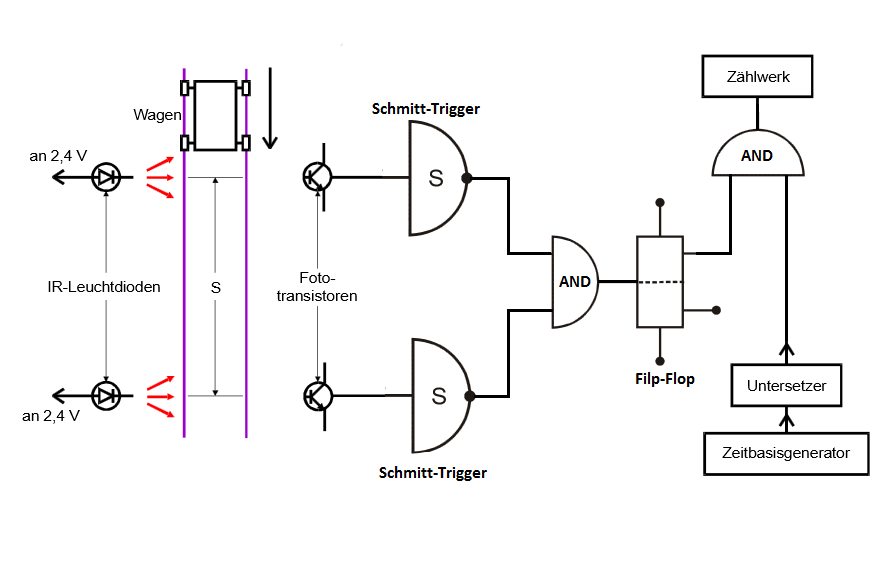
\includegraphics[width=0.7\textwidth]{Aufbau1.png}
 \caption{Aufbau zur Bestimmung der Geschwindigkeit des Wagens}
 \label{fig:geschw}
 \end{figure}\\
Zu Beginn wandeln Schmitt-Trigger die an den Phototransistoren anliegenden
Spannungen in TTL-Signale um, dies ist notwendig für die weiteren Komponenten
der Schaltung. Unterbricht der Wagen das Signal an der ersten Schranke, so
springt das Potential am $AND$-Gatter auf $L$, an diesem sind beide
Phototransistoren angeschlossen. Der Zustand der bistabilen
Kippstufe ändert sich, sodass am $Q-$Ausgang ein $H$-Potential anliegt.
Die Signale vom Zeitbasisgenerator können durch ein $AND$-Gatter
in das Zählwerk gelangen. Der Zeitbasisgenerator gibt Impulse mit einer Präzision
von $10^{-5}$ aus, dieser fungiert also als Uhr. Der  Untersetzer vermindert hier
nur die Impulse um einen einstellbaren Faktor $10^n$.
Die Entfernung der beiden Lichtschranke wird mit einem Maßband gemessen.
\newpage
\subsection{Messung der Wellenlänge}
Die Abbildung \ref{fig:schall} zeigt den Aufbau zur Bestimmung der Wellenlänge.
\begin{figure}
 \centering
 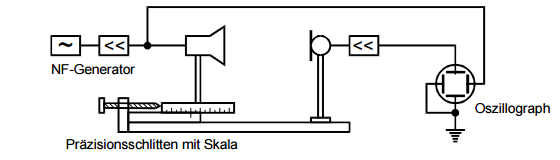
\includegraphics[width=0.7\textwidth]{schall.png}
 \caption{Aufbau zur Bestimmung der Schallgeschwindigkeit durch die Wellenlänge. \cite{skript}}
 \label{fig:schall}
 \end{figure}\\
Ein Lautsprecher wird auf einem Präzisionsschlitten montiert, diesem gegenüber ist das Mikrophon angebracht.
Das, über den Lautsprecher ausgegebene, generierte Signal und das Signal des Mikrophons werden auf das Oszilloskop gegeben.
Im XY-Betrieb entstehen Lissajous-Figuren. Sind die beiden Signale in Phase oder gegenphasig,
so wird am Oszilloskop eine Grade ausgegeben.
Der entsprechende Abstand zwischen zwei identischen Lissajous-Figuren ist dann die Wellenlänge $\lambda$.
\subsection{Frequenzmessung}
\label{sec:Frequenzmessung}
Um die Frequenzänderung bei dem Doppler-Effekt zu messen,
wird der Versuch wie in Abbildung \ref{abb:Frequenzdiff} aufgebaut.
\begin{figure}
\centering
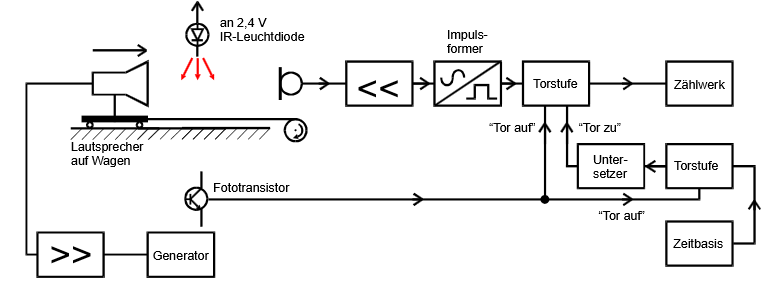
\includegraphics[width=0.7\textwidth]{Frequenzmessung.PNG}
\caption{Aufbau zur Messung der Frequenzänderung beim Doppler-Effekt.\cite{skript}}
\label{abb:Frequenzdiff}
\end{figure} \FloatBarrier
Das Mikrophon wandelt wieder das vom Lautsprecher
gesendete Signal in eine elektrische Schwingung um.
Diese wird in einen Rechteckimpuls umgewandelt und
kann nun von den digitalen
Bausteinen verarbeitet werden.
Die digitalen Bausteine werden so geschaltet,
dass das Zählwerk, die Impulse, die innerhalb
von einer Sekunde auf das Zählwerk gelangen, aufnimmt und
folglich genau die Frequenz anzeigt.
Dafür wird der Untersetzer auf $10^6$ gesetzt
und die Bausteine wie Abbildung \ref{abb:digitalF} zusammen gesetzt.
\begin{figure}
\centering
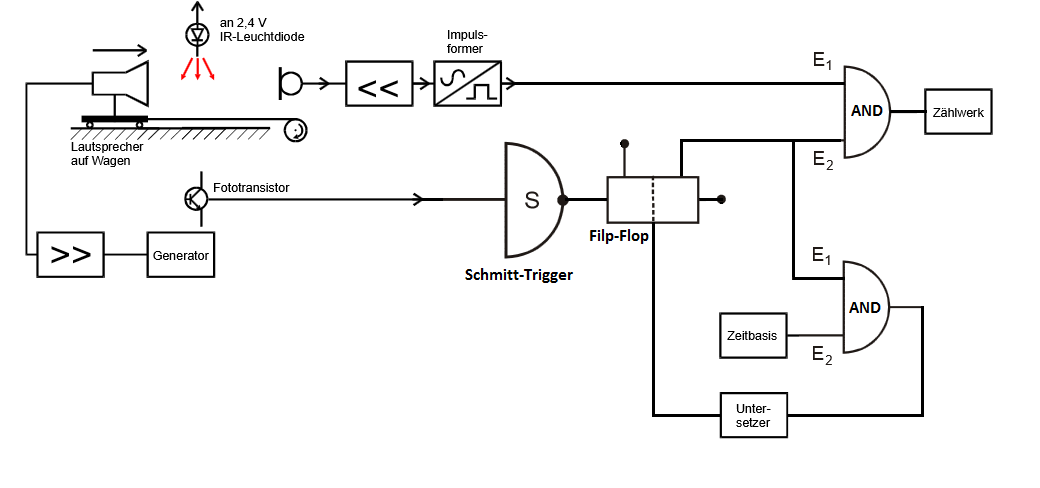
\includegraphics[width=0.7\textwidth]{digitalebausteile.png}
\caption{Aufbau der digitalen Bausteine.}
\label{abb:digitalF}
\end{figure}
\FloatBarrier
Durch diesen Aufbau löst die Lichtschranke ein Impuls
aus der dafür sorgt, dass das Zählwerk eine Sekunde
lang geöffnet wird und die Impulse des umgewandelten
Signales aufnimmt.
Die Messung besteht darin, dass der Wagen mit
dem Lautsprecher mit unterschiedlichen Geschwindigkeiten,
gegeben durch die unterschiedlichen Gänge des Synchromotors,
auf das Mikrophon zu- und
wieder  wegfährt. Jedes mal passiert dieser
die Lichtschranke und lößt die Messung des
Freuquenz aus. Dies wird für jede Geschwindigkeit
5-mal wiederholt und der Wert gemittelt. Am Anfang wird
auch die Grundfrequenz $\nu_{0}$ gemessen, indem die
Lichtschranke manuell ausgelöst wird, aber der Wagen nicht bewegt wird.
\subsection{Schwebung}
\label{sec:Schwebung}
Um die Frequenzänderung mit Hilfe der Schwebungsmethode
zu bestimmen, wird der Versuch wie in Abbildung \ref{abb:Schwebung}
aufgebaut.
\begin{figure}
\centering
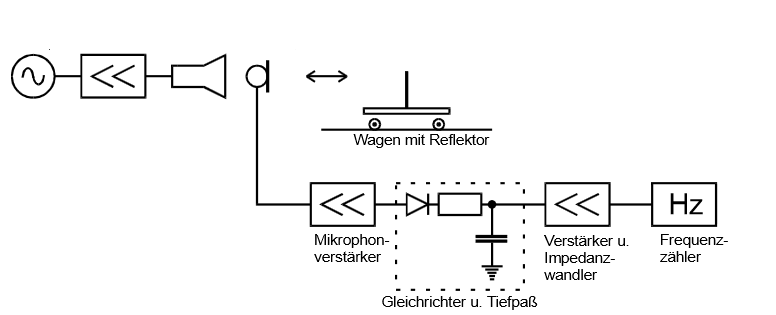
\includegraphics[width=0.7\textwidth]{Schwebung.PNG}
\caption{Aufbau zur Messung der Frequenzänderung beim Doppler-Effekt mit Hilfe der Schwebungsmethode.\cite{skript}}
\label{abb:Schwebung}
\end{figure}
Der Lautsprecher sendet wieder ein Signal aus.
Hierbei nimmt das Mikrophon nun sowohl die
Ruheschwingung des Lautsprechers, als
auch die durch den Reflektor auf dem
Wagen reflektierten Schwingungen auf.
Dieses überlagerte Signal wird durch einen Gleichrichter
und einen Tiefpass geschickt. Die Frequenz der dadurch
entstehenden Spannung wird mit einem Frequenzzähler
gemessen, der wieder durch die digialen Bausteine
aufgebaut wird. Dies wird genau wie in der Abbildung
 \ref{abb:digitalF} aus dem Kapitel \ref{sec:Frequenzmessung} realisiert.
Wieder wird der Wagen mit unteschiedichen Geschwindigkeiten
durch die Lichtschranke bewegt und die Frequenz gemessen.
